\documentclass[../manuale_sviluppatore.tex]{subfiles}

\begin{document}

\subsection{Design Pattern architetturale: MVP}
Il design pattern architetturale scelto per il prodotto è il \glossario{Model View Presenter}, di 
conseguenza le componenti principali del prodotto sono le seguenti:
\begin{itemize}
	\item \textbf{Model}: tra i model figurano tutti i tipi che hanno il compito di mantenere i dati 
	del dominio, nello specifico vi sono \emph{Dataset} (rappresentante il dataset caricato 
	nell'applicazione), \emph{DistanceMatrix} (rappresentante la matrice delle distanze associata 
	al dataset caricato)e i modelli delle visualizzazioni che preservano la configurazione delle 
	stesse;
	\item \textbf{Presenter}: tra i presenter figurano tutti i tipi che implementano la logica di 
	business e la logica di visualizzazione, in particolare vi sono i presenter delle 
	visualizzazioni, dei \glossario{components} e i manager dell'applicazione che ne gestiscono il 
	corretto funzionamento;
	\item \textbf{View}: le view sono dei tipi sostanzialmente passivi che visualizzano i dati di 
	dominio secondo la configurazione dell'applicazione, ed indirizzano gli eventi ai presenter 
	affinché essi li elaborino e producano degli aggiornamenti coerenti con li stessi; tra le view 
	vi sono il codice HTML dei grafici e i diversi tipi degli elementi di modifica dei grafici.
\end{itemize}

Nell'architettura di \emph{HD-Viz} ciascun component è composto da un presenter e da una view, 
non necessita di un modello specifico in quanto i dati dipendono dal modello dei grafici, dal 
dataset o dalla matrice delle distanze. Nel caso dei grafici invece la view viene realizzata 
tramite le funzionalità di D3.js.

\begin{figure}[H]
	\centering
	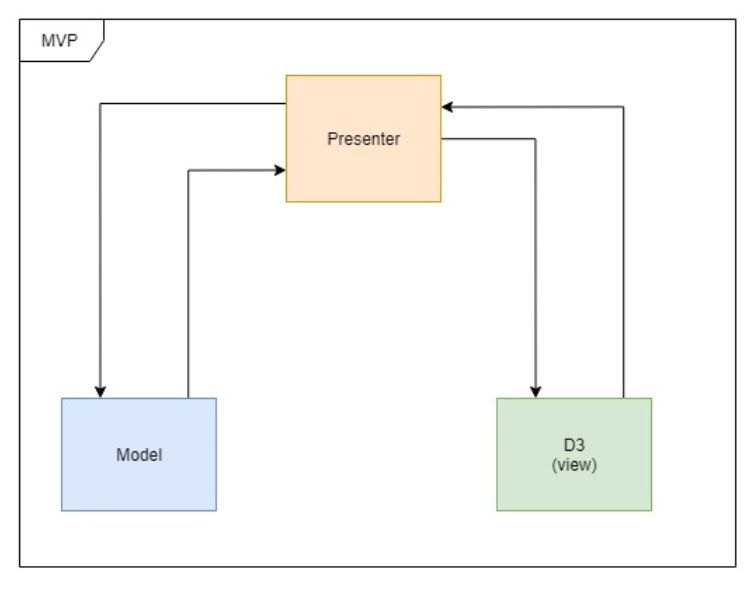
\includegraphics[width=13cm]{src/img/patternMVP.jpg}
	\caption{Pattern MVP}
\end{figure}

\subsection{Architettura di dettaglio}
\subsubsection{Client}
\label{ssub:client}

Per la definizione dei package del prodotto si è deciso di seguire il principio di progettazione 
\emph{Common Reuse Principle}, di modo da avere tipi che vengono utilizzati assieme all'interno 
dello stesso package.

\begin{figure}[H]
	\centering
	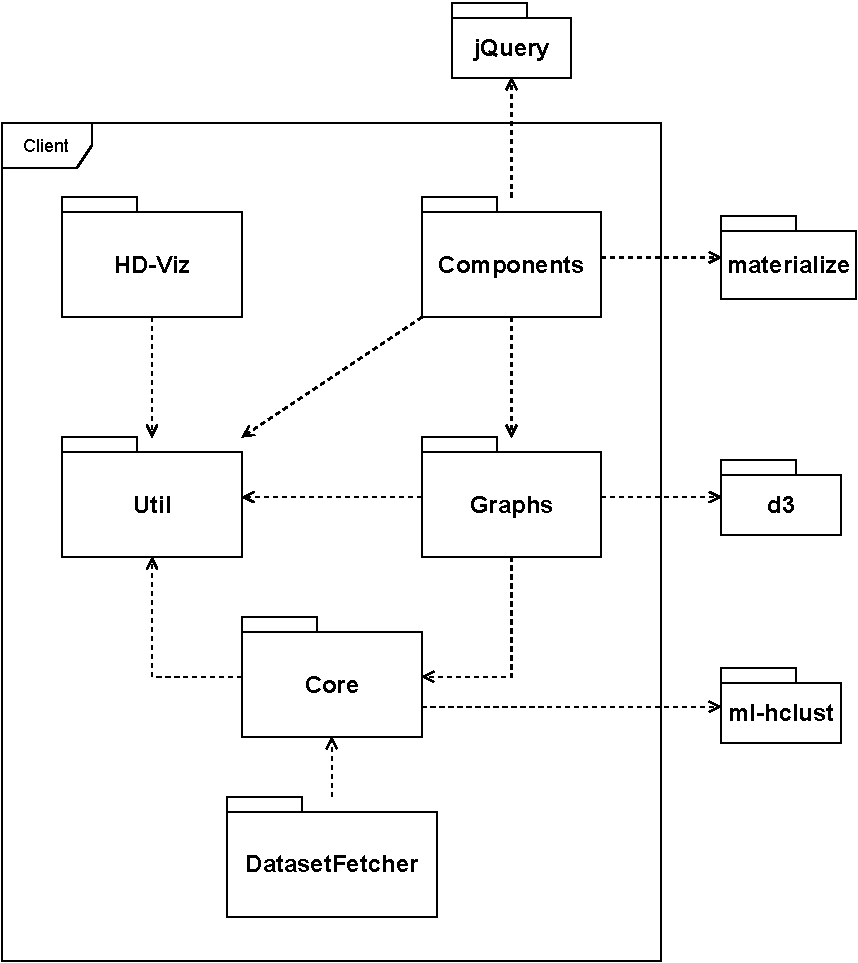
\includegraphics[width=10cm]{src/img/packageDiagramOverview.pdf}
	\caption{Struttura generale HD-Viz}
\end{figure}

I package principali sono:
\begin{itemize}
	\item \textbf{Util}: all'interno del package sono presenti tutti i tipi di supporto necessari 
	nell'applicazione, come per esempio l'implementazione del design pattern observer, largamente 
	utilizzata all'interno del prodotto;
	\item \textbf{Core}: all'interno del package vi sono tutti i tipi relativi alle strutture dati 
	cardine del prodotto, ossia il \emph{Dataset} e la \emph{DistanceMatrix};
	\item \textbf{HD-Viz}: contiene i manager, tipi che realizzano la \emph{dependency inversion} e 
	garantiscono il corretto funzionamento dell'applicazione;
	\item \textbf{Graphs}: package che contiene i tipi dei modelli, dei presenter e le view dei 
	grafici di HD-Viz;
	\item \textbf{Components}: contiene i tipi dei presenter e delle view dei diversi componenti, 
	ossia quegli elementi che si interfacciano con il \emph{Dataset}, la \emph{DistanceMatrix} o i 
	modelli dei grafici e ne modificano i dati o le proprietà di visualizzazione.
\end{itemize}

\newpage

\subsubsection*{Core}

Il package \emph{Core} presenta al suo interno i principali costituenti dei dati di dominio 
dell'applicazione, che sono anche i tipi fondamentali per il funzionamento di HD-Viz, ossia 
\emph{Dataset} e \emph{DistanceMatrix}, i quali hanno rispettivamente il compito di mantenere lo 
stato del dataset sul quale si basano le visualizzazioni e la matrice delle distanze associata al 
dataset stesso. In più vi sono numerosi tipi per gestire lo stato interno delle strutture dati, 
comportando così una restrizione maggiore delle resonsabilità di ciascun tipo. All'interno del 
package viene fatto un largo uso del design pattern observer per la notifica delle modifiche 
effettuate sulle strutture dati da cui dipendono le visualizzazioni, infatti \emph{Dataset}, 
\emph{DistanceMatrix} e \emph{Dimension} implementano il tipo astratto \emph{Subject}, mentre 
\emph{Dataset} e \emph{DistanceMatrix} implementano l'interfaccia \emph{Observer}. Inoltre è 
presente la realizzazione del design pattern strategy per la scelta della tipologia di distanza da 
utilizare per il calcolo della matrice delle distanze.

\begin{figure}[H]
	\centering
	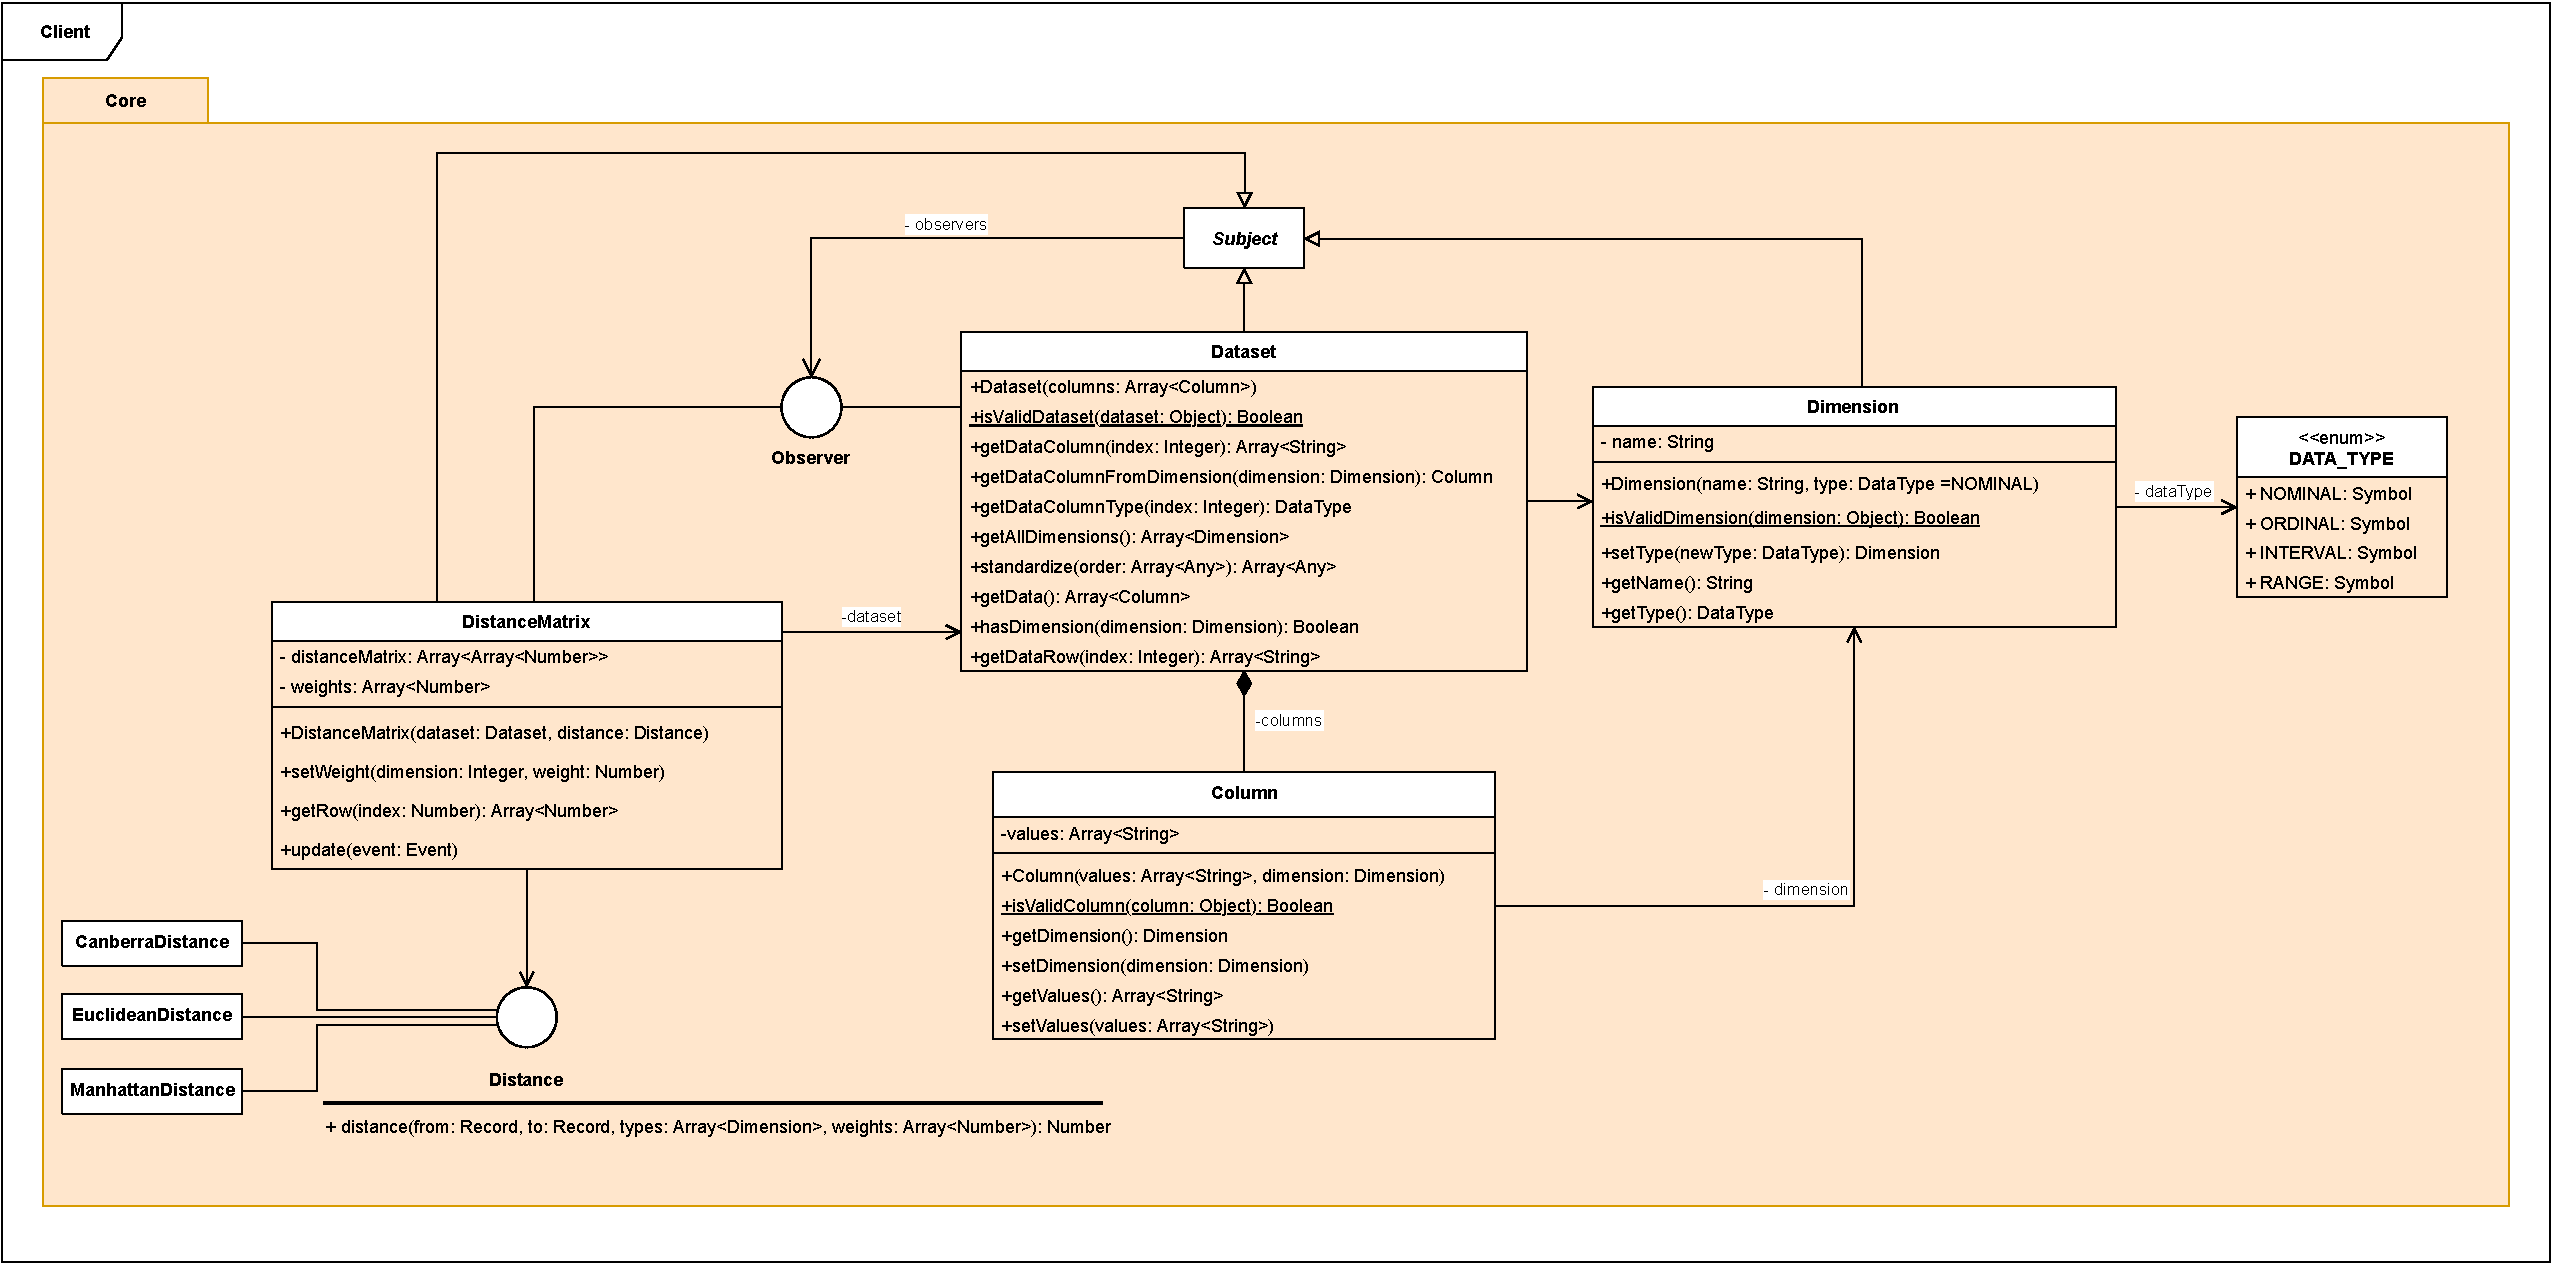
\includegraphics[width=18cm]{src/img/core.pdf}
	\caption{Diagramma delle classi del package Core}
\end{figure}

\subsubsection*{HD-Viz}

All'interno del package HD-Viz sono presenti diversi tipi \emph{manager} che realizzano la 
\emph{dependency injection} e gestiscono funzionalità di alto livello. Il tipo \emph{HDVizmanager} 
a livello logico è il nucleo dell'applicazione infatti si occupa di tener traccia dei dati per 
evitare istanze multiple del \glossario{Dataset}, della \emph{DistanceMatrix} e dei grafici una 
volta creati. Nel momento in cui viene modificato il dataset originale per modificare le 
visualizzazioni, esso funge da tramite creando una copia del dataset e usando quest'ultima per le 
modifiche, cosicchè il dataset originale resti invariato.
Tra gli altri manager vi sono \emph{GraphCreatorManager} che gestisce le factories per la 
creazione dei vari modelli dei grafici. Il \emph{CurrentGraphManager} verifica se le factories sono 
in grado di costruire il grafico, quindi si occupa di comunicare con il presenter e il modello del 
grafico relativo.

\subsubsection*{Graphs}

Il package Graphs presenta al suo interno un sottopackage per visualizzazione; ciascun sottopackage 
presenta un tipo \emph{model} ed un tipo \emph{presenter}. Il primo estende \emph{GraphModel}, che 
a sua volta estende \emph{Subject} e implementa \emph{Observer} ed ha il compito di gestire la 
configurazione della visualizzazione, il modello della visualizzaizone inoltre implementa diverse 
interfacce, congrue alle  funzionalità ed alla tipologia della visualizzazione stessa. Il 
\emph{presenter} invece estende \emph{GraphPresenter}, il quale implementa \emph{Observer}, ed ha 
il compito di gestire le proprietà grafiche della visualizzazione oltre che generare la 
vista grazie a D3.js.

\begin{figure}[H]
	\centering
	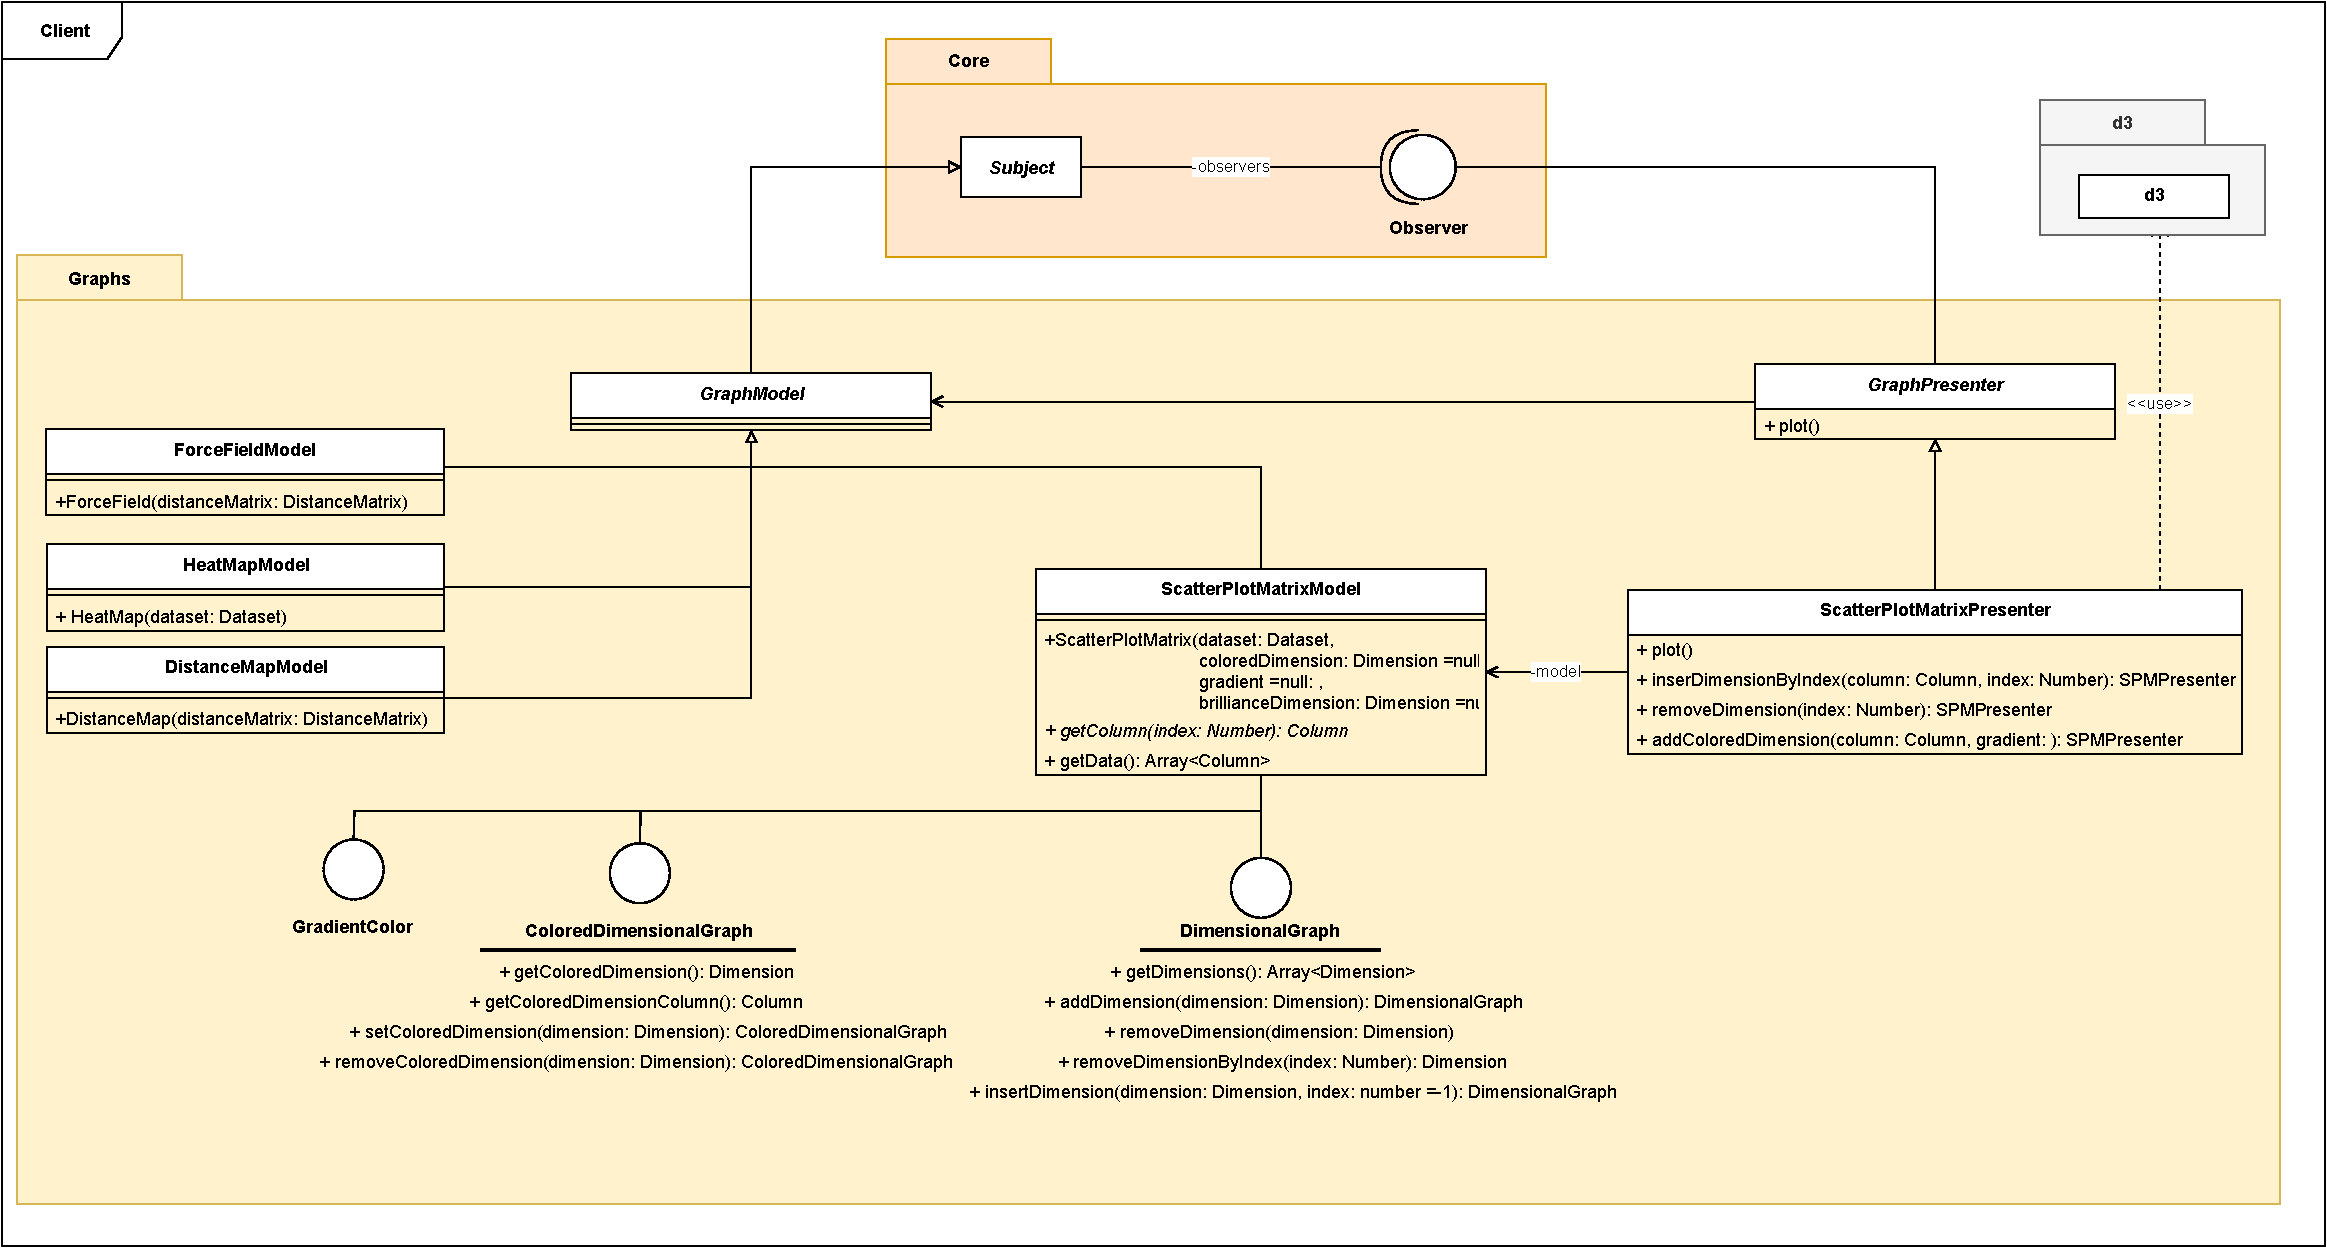
\includegraphics[width=18cm]{src/img/graphs.pdf}
	\caption{Diagramma delle classi del package Graphs}
\end{figure}


\subsubsection*{Components}

Il package Components racchiude al suo interno tutti i diversi components; ciascuno di essi è 
costituito da un presenter ed una view. Il primo estende \emph{Subject} ed implementa 
\emph{Observer}, gestisce la logica per effettuare le modifiche nei modelli delle visualizzazioni e/o 
sulle strutture dati di Core; la view invece presenta semplicemente il codice HTML del component e 
lega metodi del presenter a determinate azioni sull'interfaccia utente.

\begin{figure}[H]
	\centering
	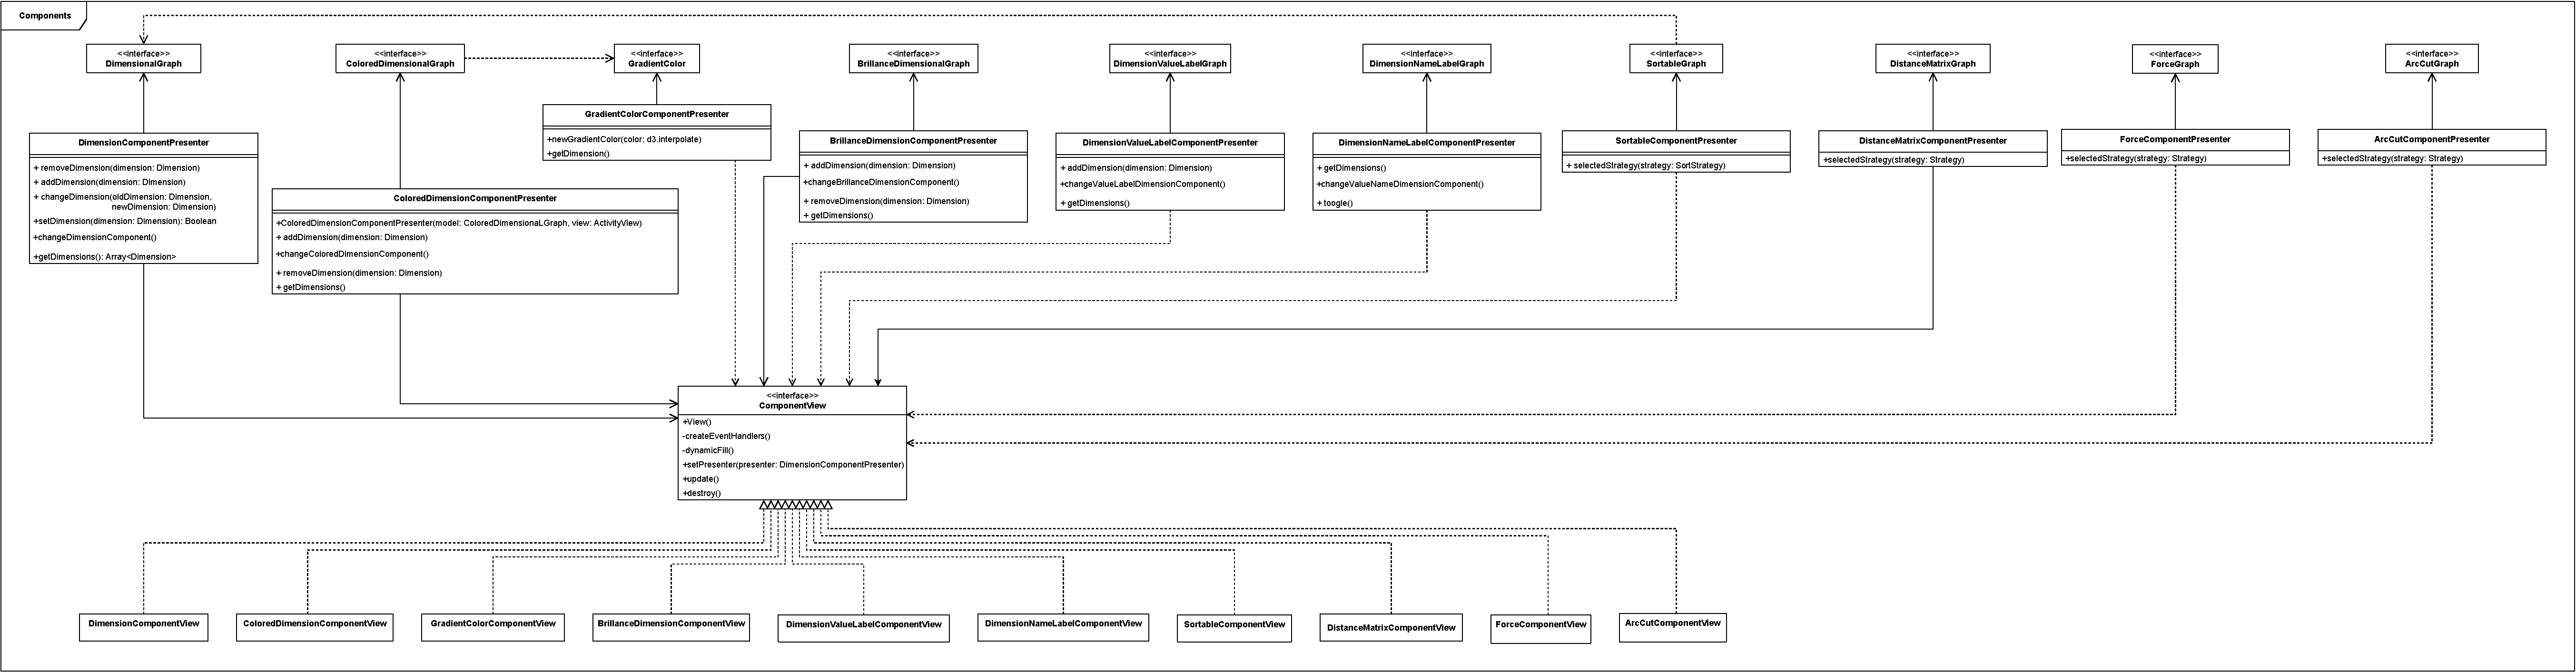
\includegraphics[width=18cm]{src/img/components.pdf}
	\caption{Diagramma delle classi del package Components}
\end{figure}

\subsubsection{Server}
\label{ssub:server}

Il lato server dell'applicativo è stato realizzato mediante l'uso del framework \emph{Express}, che 
si occupa della creazione e gestione di un servizio HTTP. \\
\emph{Express} fornisce un particolare modulo, \emph{Router}, con il quale è possibile definire dei 
percorsi al fine di gestire delle richieste HTTP indipendentemente dalla implementazione del server. 
Questo rende possibile accordarli all'applicativo express finale.

\par dal seguente diagramma di package si possono riconoscere diversi package, di cui segue la 
descrizione.\\

\begin{figure}[H]
	\centering
	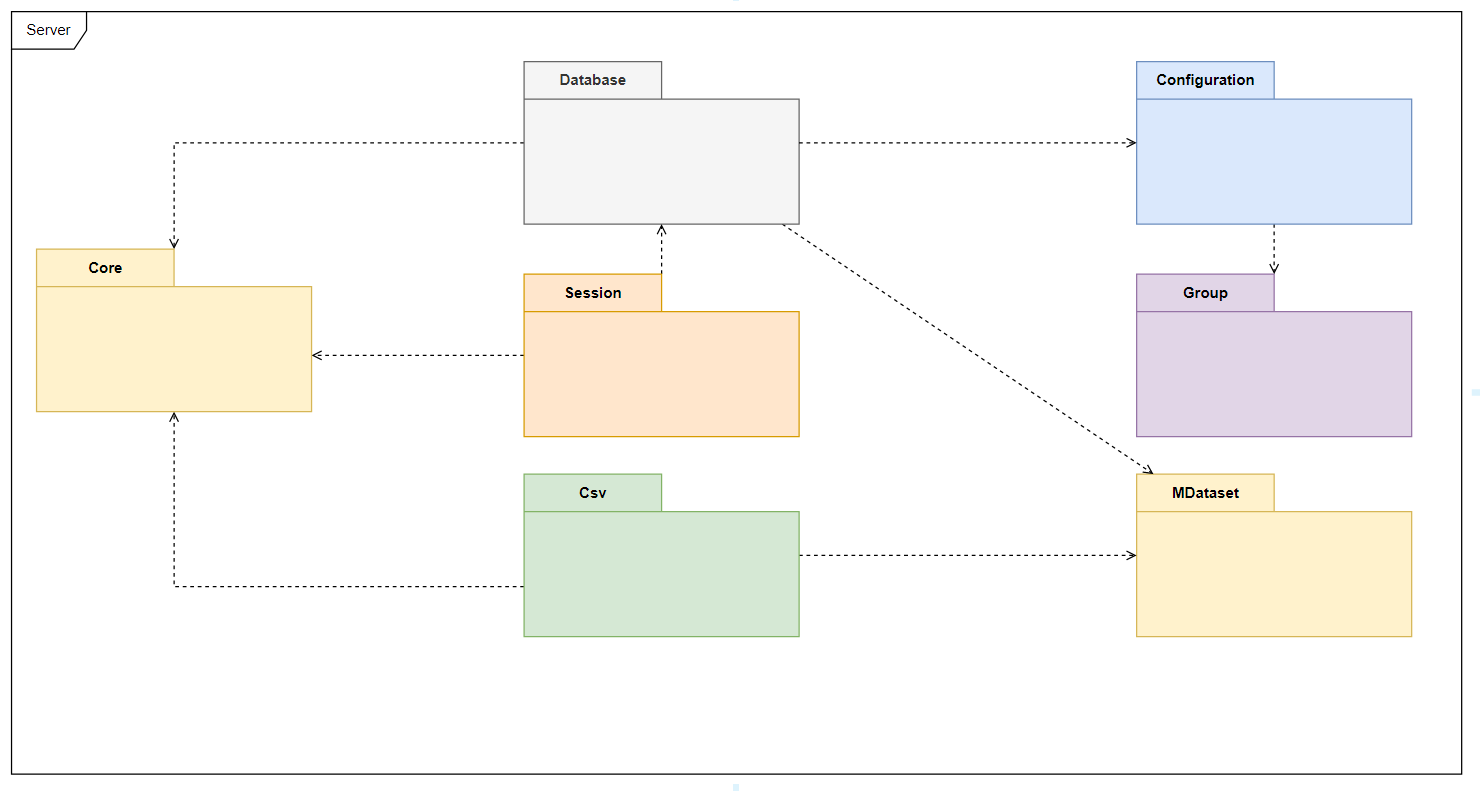
\includegraphics[width=18cm]{src/img/package-server.png}
	\caption{Diagramma package lato server.}
\end{figure}

\textbf{NB}: Al fine di rendere la comprensione più chiara, vengono riportati frammenti dei diversi 
diagrammi delle classi. Verranno quindi omesse le parti considerate non significative.
\newpage

\begin{itemize}
	
	\item \textbf{Core:} Nucleo dell'applicativo, contiene le classi per la gestione del server
	e la definizione di nuovi percorsi da creare mediante la classe astratta \emph{Route}. 
	
	La classe App definisce il funzionamento del server al quale è possibile accordare le 
	possibili implementazioni di \emph{Route} e, solamente in costruzione, i possibili 
	percorsi statici che devono essere resi accessibili. 
	
	\emph{Application} si occupa inoltre della generazione di un ambiente dotato di sessione. Essa 
	si basa sull'uso delle librerie esterne \emph{express-session} e \emph{memorystore} che 
	combinate, creano uno store virtuale di oggetti memorizzati di tipo \emph{DataSession}, per ogni 
	utente che accede al servizio.
		
	\begin{figure}[H]
		\centering
		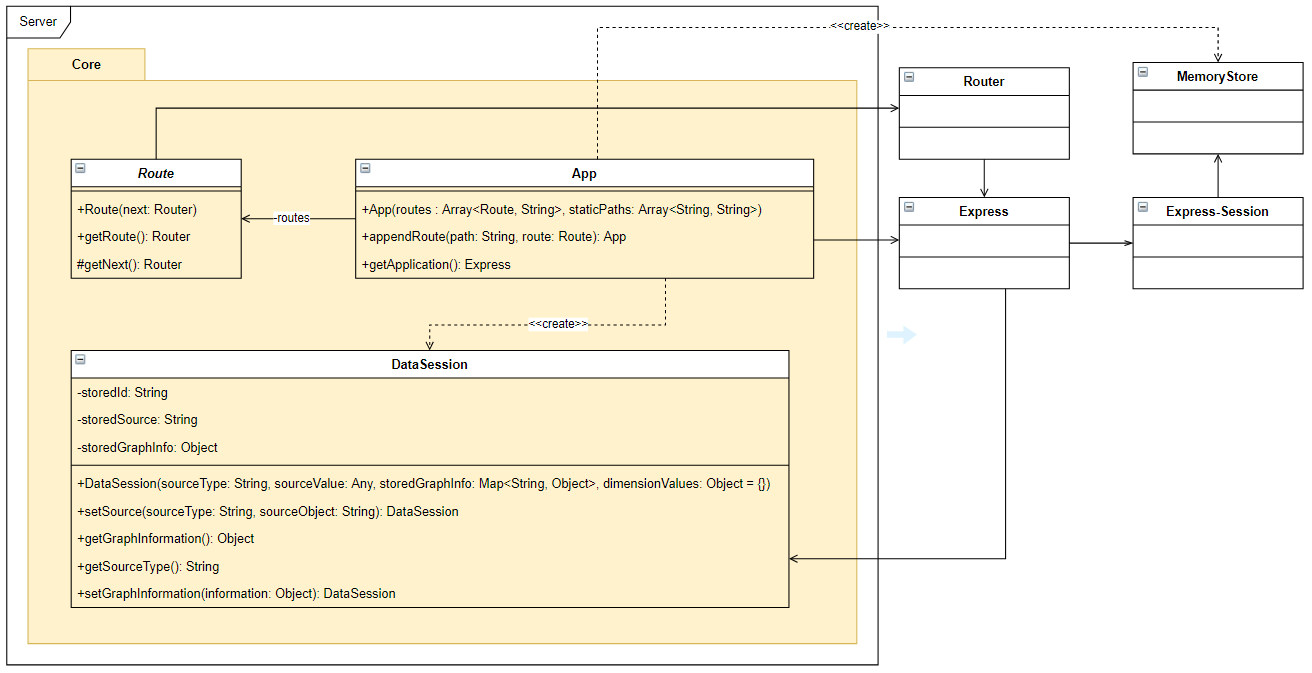
\includegraphics[width=18cm]{src/img/server-core.png}
		\caption{Classi del package di Core}
	\end{figure}

	\newpage
	\item \textbf{Csv:} Package per la gestione di file csv caricati da client. 
	
	Le richieste HTTP vengono gestite dalla \emph{CsvRoute} che realizza la classe astratta 
	\emph{Route}.
	
	L'elaborazione, che ricade nella classe \emph{CsvApplication}, avviene mediante l'uso della 
	libreria \emph{fs} di Node.js per la lettura del file dato in input. La classe crea una 
	rappresentazione temporanea del dataset al fine di spedire al client un risultato già 
	manipolabile, creando quindi un \emph{MDataset}.
	
	\begin{figure}[H]
		\centering
		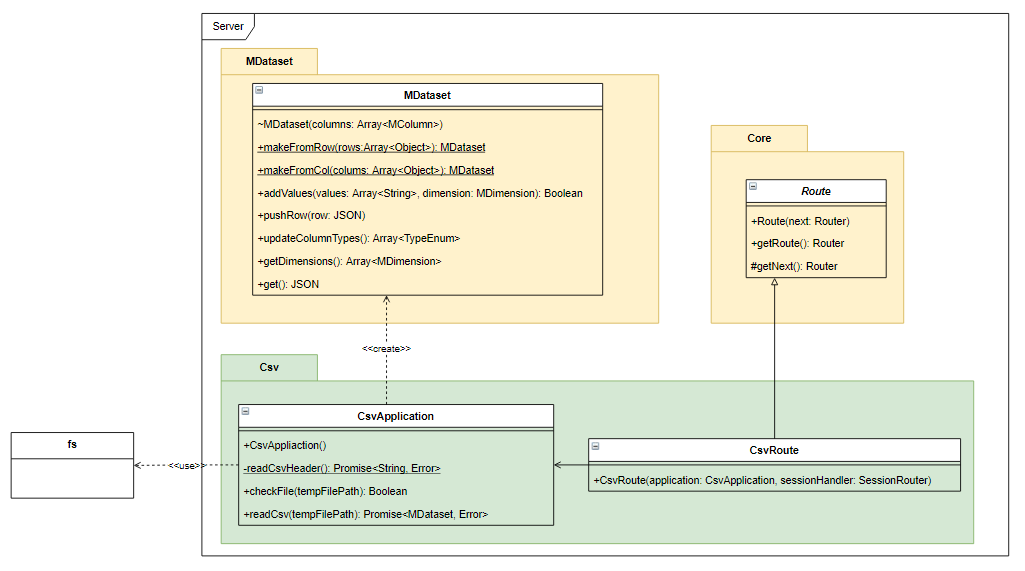
\includegraphics[width=18cm]{src/img/server-csv.png}
		\caption{Classi del package di Csv}
	\end{figure}

	\newpage
	\item \textbf{Database:} Il package per il reperimento dei dati da un database su un dato server.
	
	Il funzionamento si basa sull'uso di configurazioni che vengono date in costruzione alla classe \emph{RelationalDbApplication} 
	che permettono di eseguire query sui database dalle informazioni date, sfruttando l'ORM Sequelize. 
	
	Dalla query eseguita sul server si costruisce un \emph{MDataset} che viene rispedito al client. 

	Tutte le operazioni, come per il package di \emph{Csv}, vengono generate da richieste HTTP entranti alla \emph{Route} del package, 
	in questo particolare caso \emph{RelationalDbRoute}.

	\begin{figure}[H]
		\centering
		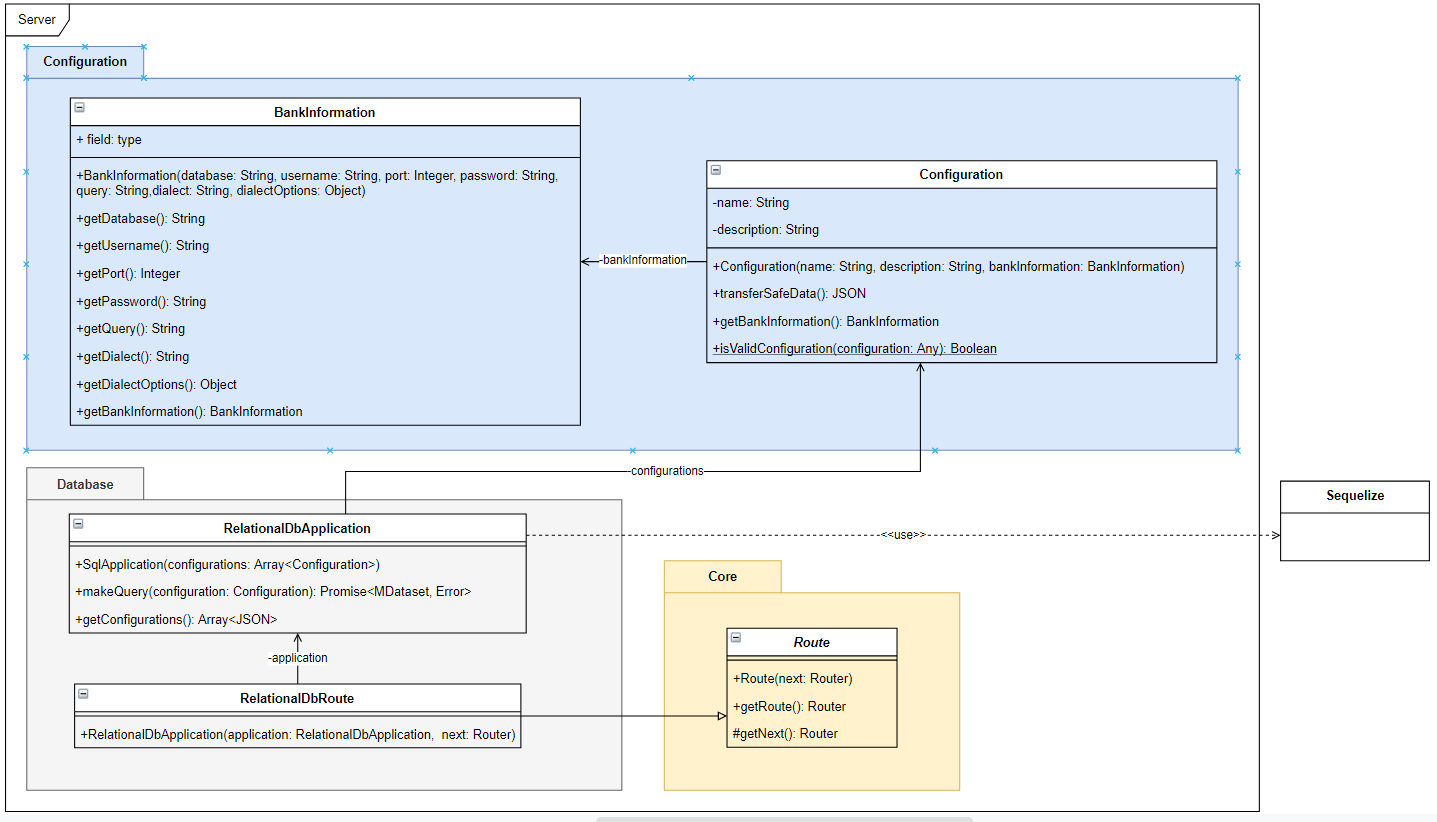
\includegraphics[width=18cm]{src/img/server-database.png}
		\caption{Classi del package di Database}
	\end{figure}


	\newpage
	\item \textbf{Configuration e Group:} Il package di Group contiene delle classi per il controllo di gruppi
	di file con lo stesso nome ma diversa estensione in un determinato percorso. Questo si presta al reperimento delle 
	configurazioni per accedere ad un database, che sono divise in un file .json e uno .sql, per la query. 

	Il \emph{Configuration Collector} dato un \emph{Group} è in grado di ricostruire le \emph{Configuration} che 
	è una rappresentazione di tutte le informazioni necessarie per accedere ad una determinata fonte di dati.
	
	\begin{figure}[H]
		\centering
		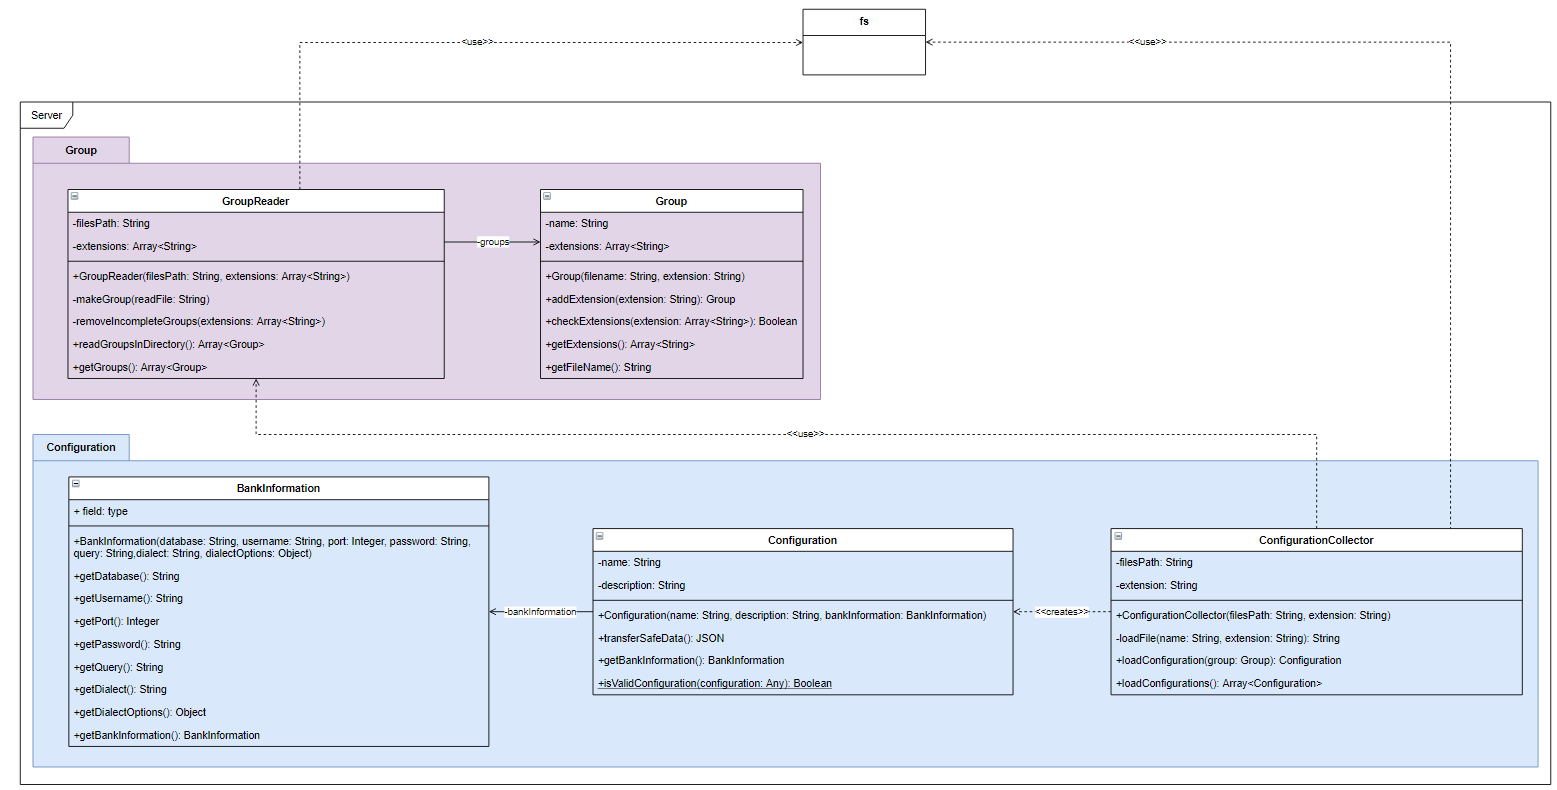
\includegraphics[width=18cm]{src/img/server-group.png}
		\caption{Classi del package di Configuration e Group}
	\end{figure}

	\item \textbf{MDataset:} Package contenente una rappresentazione in versione minimale, priva quindi delle funzionalità del dataset
	che viene calcolato lato server e spedito al client, in particolare usate dai package \emph{Csv, Database}.

	\item \textbf{Session:} Package che contiene la classe per la gestione ed il mantenimento della sessione per ogni utente che 
	accede al servizio di HdViz. Esso permette di ottenere informazioni sulla propria \emph{DataSession} o di memorizzare delle 
	modifiche avvenute a lato client sulla sessione.

\end{itemize}
\end{document}